
\documentclass[ms.tex]{subfiles}
\begin{document}

\section{Results}
\label{sec:results}

% {\color{red}
In this section, we present the predictions of our GCE models.
We establish a fiducial model in~\S~\ref{sec:results:fiducial}, which adopts
$\ycc{N} = 3.6\times10^{-4}$ and our linear AGB star yields (equation
\ref{eq:linear_yield}) with~$\xi = 9\times10^{-4}$ along with the O and Fe
yields of~\citet[see discussion in~\S~\ref{sec:yields}]{Johnson2021}.
% Although we presented this parametrization in comparison to
% the~\cristallo~yields with~$\xi = 3\times10^{-4}$ in
% Fig.~\ref{fig:agb_yield_models}, we find that a renormalization is necessary to
% reproduce the~\ohno~relation as observed; we discuss this point further
% in~\S~\ref{sec:results:yields}.
We discuss the evolution of this model in radius and time as well as the impact
of stellar migration.
% Within this fiducial model, we demonstrate the impact of stellar migration on
% N enrichment rates by making use of the diffusion migration prescription
% (see discussion in~\S~\ref{sec:multizone}).
In~\S~\ref{sec:results:yields}, we consider AGB star yield models taken from
the literature (see discussion in~\S~\ref{sec:yields:agb}) and use an
empirical~\ohno~relation to discriminate among them.
For each of these previously published yields, we explore alternate
parametrizations of our SN yields and/or the efficiency of outflows which may
address their shortcomings in reproducing the observed trend.
We return to the fiducial model in~\S~\ref{sec:results:t_z_dep_comp} to
demonstrate the dominance of the metallicity dependence of N yields over the
AGB star DTD in establishing the gas-phase~\ohno~relation.
To make the comparisons more clear, we make use of the post-processing
migration prescription in~\S\S~\ref{sec:results:yields}
and~\ref{sec:results:t_z_dep_comp} but otherwise retain the diffusion
prescription (see discussion in~\S~\ref{sec:multizone}).
In~\S~\ref{sec:results:vincenzo_comp}, we compare our fiducial~\no~vs. age
and~\no~vs.~\ofe~trends to the stellar abundances derived from APOGEE data
by~\citet{Vincenzo2021}.
In~\S~\ref{sec:results:schaefer_comp}, we demonstrate how variations in the
SFE or inflow rate can induce scatter in the gas-phase~\ohno~relation.
We finish presenting our results in~\S~\ref{sec:results:ohno_equilibrium} by
offering an analytic understanding of the~\ohno~relation obtained with
chemical equilibrium arguments inspired by~\citet{Weinberg2017}.
As a reference for the reader, in Table~\ref{tab:resultsref} we provide a
summary of which migration prescriptions we take as a default and which AGB
star yield models we consider in each subsequent subsection.
% }

\subsection{Evolution of a Fiducial Model}
\label{sec:results:fiducial}

% fig 5
\begin{figure*}
\centering
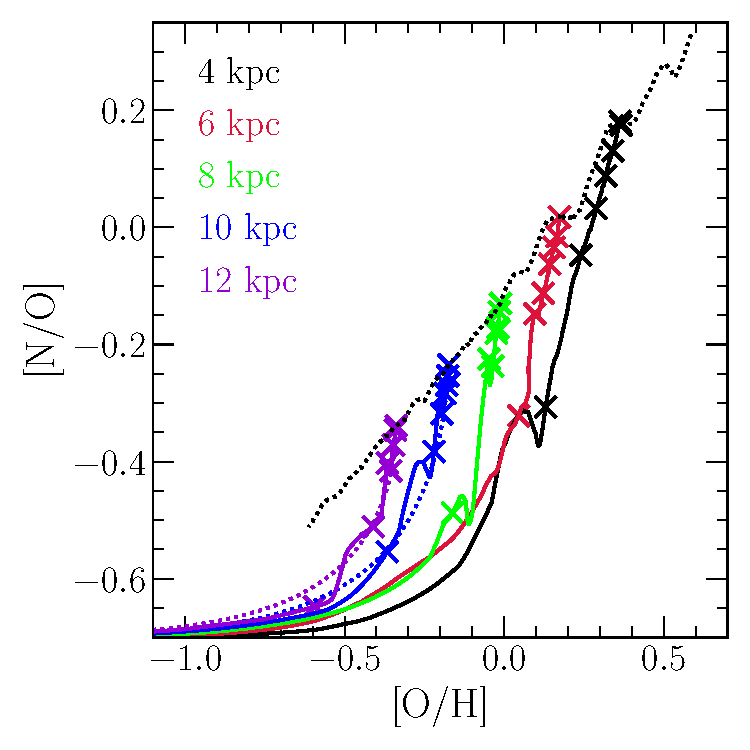
\includegraphics[scale = 0.6]{no_oh_superposition.pdf}
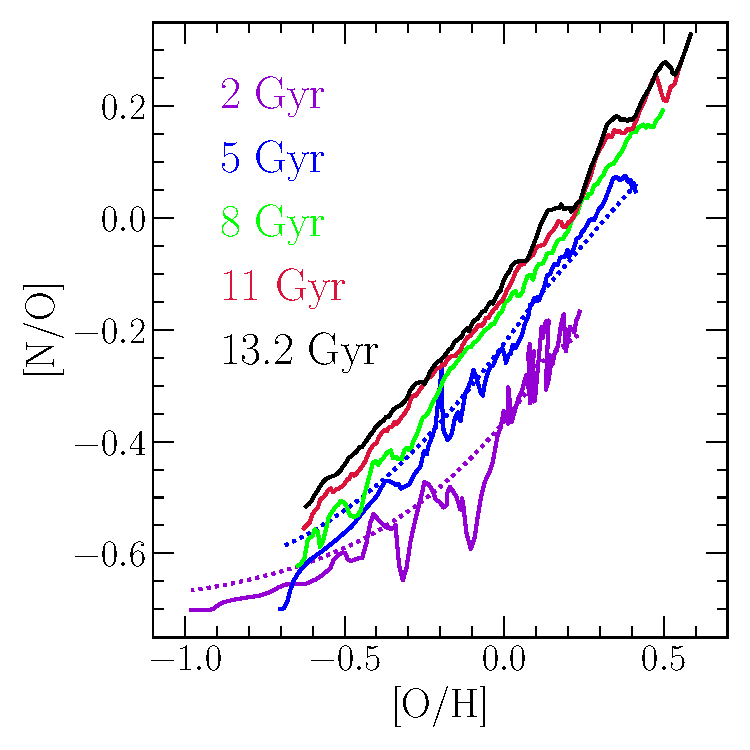
\includegraphics[scale = 0.6]{no_oh_timeevol.pdf}
\caption{
\textbf{Left}: The gas-phase~\ohno~relation parametrized by time at
fixed radius (solid coloured lines) in the fiducial model. X's denote the
abundances at~$t = 2$, 4, 6, 8, 10, 12, and 13.2 Gyr (the present day) at all
radii.
The dotted black line is the same as the solid black line in the right panel.
Coloured dotted lines mark the evolution of our model at~$\rgal = 10$ and 12
kpc when we neglect the impact of stellar migration on enrichment rates (i.e.
the ``post-processing'' migration prescription from~\citealp{Johnson2021}; see
discussion in~\S~\ref{sec:multizone}).
\textbf{Right}: The gas-phase~\ohno~relation parametrized by radius at
various snapshots (solid coloured lines) in our fiducial model.
Similar to the left panel, coloured dotted lines denote the resulting relation
at~$t = 2$ and 5 Gyr when we neglect stellar migration in computing enrichment
rates.
}
\label{fig:no_oh_timeevol}
\end{figure*}

% {\color{red} [Redacted paragraph incorporated into the one above]}
% Our fiducial model adopts~$\ycc{N} = 3.6\times10^{-4}$ and our linear AGB star
% yield model (equation~\ref{eq:linear_yield}) with~$\xi = 9\times10^{-4}$
% along with the O and Fe yields of~\citet[][see discussion
% in~\S~\ref{sec:yields}]{Johnson2021}.
% Although we presented this parametrization in comparison to
% the~\cristallo~yields with~$\xi = 3\times10^{-4}$ in
% Fig.~\ref{fig:agb_yield_models}, we find that a renormalization is necessary to
% reproduce the~\ohno~relation as observed; we discuss this point further
% in~\S~\ref{sec:results:yields}.
% To demonstrate the impact of stellar migration on N enrichment rates, we make
% use of the diffusion migration prescription in this section (see discussion
% in~\S~\ref{sec:multizone}).
% {\color{red}
% As a reference for the reader, in Table~\ref{tab:resultsref} we provide a
% summary of which migration prescriptions and which AGB star yield models we
% take as default in each subsection of~\S~\ref{sec:results}.
% }
\par
In the left panel of Fig.~\ref{fig:no_oh_timeevol}, we plot the evolution of N
and O abundances in the gas phase at five different Galactocentric radii
in our fiducial model (see paragraph above).
% {\color{red} in our fiducial model (see paragraph above)}.
At early times,~\oh~is low and~\no~reflects the ratio of the CCSN yields
(\no\subcc~$\approx -0.7$).
Consequently, the tracks in each ring are similar.
Once lower mass stars begin to evolve through an AGB phase, they enrich the
ISM with N but negligible amounts of O, increasing~\no.
At this point, the tracks in each ring separate from one another.
This separation is a consequence of the metallicity gradient in~\oh~being
established early in the Galaxy's evolution.
The radial gradient in our model arises out of a decrease in the equilibrium
abundance of O with increasing radius.
Produced on short timescales by CCSNe, O achieves equilibrium faster than
elements produced by delayed nucleosynthetic sources~\citep{Weinberg2017}.
% At this point, the tracks in each ring separate from one another.
% This separation is a consequence of the metallicity gradient in~\oh~being
% established early in the Galaxy's evolution.
% Being an element produced primarily by CCSNe on short delay times, O reaches
% an equilibrium abundance before elements produced by delayed nucleosynthetic
% sources~\citep{Weinberg2017}.
The ISM therefore reaches equilibrium in O soon after AGB stars begin
producing N, after which~\no~continues to increase at an approximately
fixed~\oh~at all radii (see also Fig.~\ref{fig:nh_feh_vs_lookback} and
associated discussion in~\S~\ref{sec:results:vincenzo_comp}).
The separation of these evolutionary tracks contests the popular interpretation
that the~\ohno~relation arises as an evolutionary sequence, instead suggesting
a superposition of evolutionary endpoints at equilibrium values set by
different outflow efficiencies.
Similar arguments have been made regarding low [$\alpha$/Fe] disc
stars~\citep[e.g.][]{Schoenrich2009, Nidever2014, Buck2020, Sharma2021}.
In short, a given ring in our model does not evolve along the~\ohno~relation,
instead following this ``rightward-then-upward'' trajectory dictated by the
timescales on which N and O achieve equilibrium.
% The N and O abundances of the Galaxy in the past therefore differ from that
% which would be derived observationally by taking their values at the present
% day from all rings (shown by the black dotted line, see discussion below).
% This contests the popular assumption that the~\ohno~relation in Milky Way-mass
% galaxies arises as an evolutionary sequence, instead suggesting a superposition
% of endpoints like that previously suggested for low [$\alpha$/Fe] disc stars
% \citep[e.g.][]{Schoenrich2009, Nidever2014, Buck2020, Sharma2021}.

\begin{table}
\caption{
A reference on which migration prescription (see~\S~\ref{sec:multizone}) we
take as a default and which AGB star yield model(s) we consider in each
subsection of~\S~\ref{sec:results}.
Our linear AGB star yield is defined in equation~\refp{eq:linear_yield}.
We use a metallicity-independent IMF-averaged massive star yield of
$\ycc{N} = 3.6\times10^{-4}$ throughout, exploring alternate,
metallicity-dependent parametrizations in~\S~\ref{sec:results:yields:yncc} only
(right panel of Fig.~\ref{fig:no_oh_predictions}).
We do not present multi-zone GCE models
in~\S\S~\ref{sec:results:yields:summary} and~\ref{sec:results:ohno_equilibrium}.
}
\begin{tabularx}{\columnwidth}{l @{\extracolsep{\fill}} l r}
\hline
Section & AGB Star Yield Model(s) & Migration Prescription
\\
\hline
\ref{sec:results:fiducial} & Linear &
Diffusion
\\
\ref{sec:results:yields} & \cristallo,~\ventura,~\karakasten,~\karakas &
Post-processing
\\
\ref{sec:results:yields:variations} & Linear,~\cristallo,~\ventura &
Post-processing
\\
\ref{sec:results:yields:yncc} & \karakasten,~\karakas & Post-processing
\\
\ref{sec:results:yields:summary} & N/A & N/A
\\
\ref{sec:results:t_z_dep_comp} & Linear & Post-processing
\\
\ref{sec:results:vincenzo_comp} & Linear & Diffusion
\\
\ref{sec:results:schaefer_comp} & Linear & Diffusion
\\
\ref{sec:results:ohno_equilibrium} & N/A & N/A
\\
\hline
\end{tabularx}
\label{tab:resultsref}
\end{table}

Because there is a delay between a stellar population's formation and N
production from its AGB stars ($\sim$250 Myr in this model; see Fig.
\ref{fig:ssp}), stellar migration can in principle occur within this time
interval.
Although the bulk of migration occurs on longer timescales, this characteristic
delay is comparable to the dynamical time of the Milky Way and is thus adequate
for kinematic heating to at least begin.
In zoom-in hydrodynamical simulations from the FIRE\footnote{
	\url{https://fire.northwestern.edu}
} suite~\citep{Hopkins2014},~\citet{El-Badry2016} find that stars in a
M$_\star \approx 10^{10.6}~\msun$ galaxy can migrate~$1 - 2$ kpc within 1 Gyr
of their formation.
Consequently, N enrichment rates at fixed~\rgal~may differ significantly from
their expected values given the SFH at that radius because stellar migration
induced a deficit or surplus of N-producing AGB stars.
These tracks can thus move vertically in the~\ohno~plane in response to AGB
stars moving between rings as the Galaxy evolves, producing the ``jitter'' in
these evolutionary tracks.
We demonstrate this effect by comparing the solid blue and purple lines to
their dotted counterparts.
These are the tracks we compute using the post-processing migration
prescription which eliminates the impact of migration on enrichment rates (see
discussion in~\S~\ref{sec:multizone}).
\par
In the right panel of Fig.~\ref{fig:no_oh_timeevol}, we plot the
gas-phase~\ohno~relation predicted by the model at various snapshots.
To obtain this, we simply take the N and O abundances in the ISM at a given
output time for each~$\delta\rgal = 100$ pc ring at~$\rgal > 2$ kpc and plot
them as a line.
The relation is generally time-independent at~$t \gtrsim 5$ Gyr.
Although there is some slight evolution toward higher~\no, the total change
in~\no~over this time interval is well within the intrinsic scatter derived
observationally (see Fig.~\ref{fig:no_oh_observed}).
Even at~$t = 2$ Gyr, corresponding to~$z \approx 2.6$,~\no~at fixed~\oh~is
only~$\sim$0.2 dex lower than its value at the present day.
Especially when considering the intrinsic scatter that would arise if we were
to consider models with, e.g., different SFHs, this calculation supports
previous arguments that the redshift evolution of the~\ohno~relation is
minimal~\citep{Vincenzo2018, HaydenPawson2021}.
\par
We again demonstrate the impact of stellar migration in the right panel of
Fig.~\ref{fig:no_oh_timeevol} by comparing the blue and purple solid lines
to their dotted counterparts, which quantify the relation using the
post-processing migration prescription.
This indicates that the local jitter seen in the relation at a given time is
a consequence of migration as discussed above.
The mechanism by which stellar migration imposes these features in
the~\ohno~plane is qualitatively similar to what~\citet{Johnson2021} find for
SN Ia production of Fe.
They found that the SN Ia rate in this model can vary by as much as a factor of
$\sim$3 at large radii ($\rgal \gtrsim 9$ kpc).
When a deficit or surplus of SN Ia events is sustained for timescales
comparable to the depletion time of the local ISM, the gas-phase abundance of
Fe increases or decreases accordingly.
As a consequence, some of the stellar populations that form during these
events are Fe-poor enough to present as young stars ($\lesssim$ 6 Gyr) with
significantly super-solar [$\alpha$/Fe] ratios, some of which are indeed
observed in the solar neighbourhood with APOGEE\footnote{
	Although some of these stars appear to have mis-labeled ages
	\citep{Jofre2016, Yong2016, Izzard2018, SilvaAguirre2018, Miglio2021}, this
	phenomenon could explain an intrinsically young sub-component
	(\citealp{Hekker2019}; see discussion in~\S\S~3.1 and 3.4 of
	\citealp{Johnson2021}).
}~\citep{Chiappini2015, Martig2015, Martig2016, Warfield2021}.
In the case of N, the effect is smaller ($\lesssim$0.1 dex in~\no) because our
model predicts N yields to be ejected from stellar populations~$\sim$5
times faster than Fe (Fig.~\ref{fig:ssp}).
Consequently, there is less time for stellar migration to occur within the
timescale of N production than there is within the timescale of Fe production.
\par
% {\color{red}
To assess how well our model characterizes N production in the Milky Way and
external galaxies, in the next section we compare the
present-day~\ohno~relation (solid black line in the right panel of
Fig.~\ref{fig:no_oh_timeevol}) to the~\citet{Dopita2016} trend.
We do the same for our AGB yield models taken from the literature
(see discussion in~\S~\ref{sec:yields:agb}), exploring variations of other
model parameters which may address their shortcomings.
We then return to our fiducial model thereafter for additional tests against
observed data.
% }


\subsection{Comparison to Observed Gas-Phase Trends}
\label{sec:results:yields}

% fig 6
\begin{figure*}
\centering
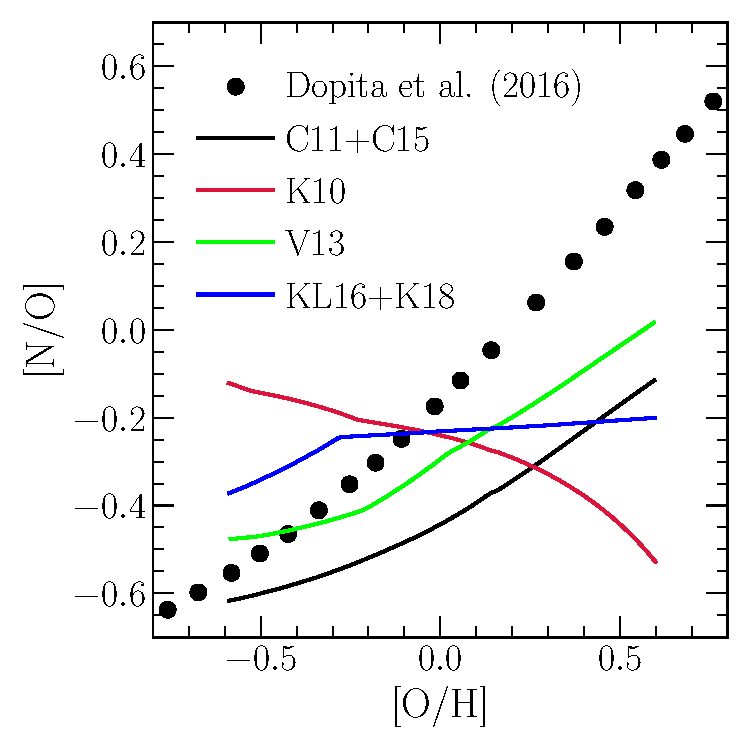
\includegraphics[scale = 0.45]{no_oh_predictions_unmodified.pdf}
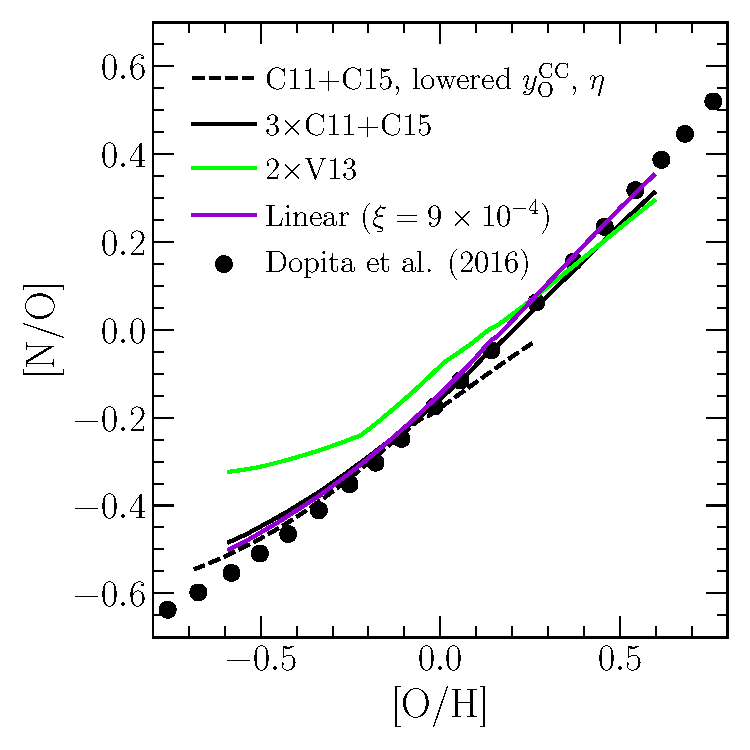
\includegraphics[scale = 0.45]{no_oh_predictions.pdf}
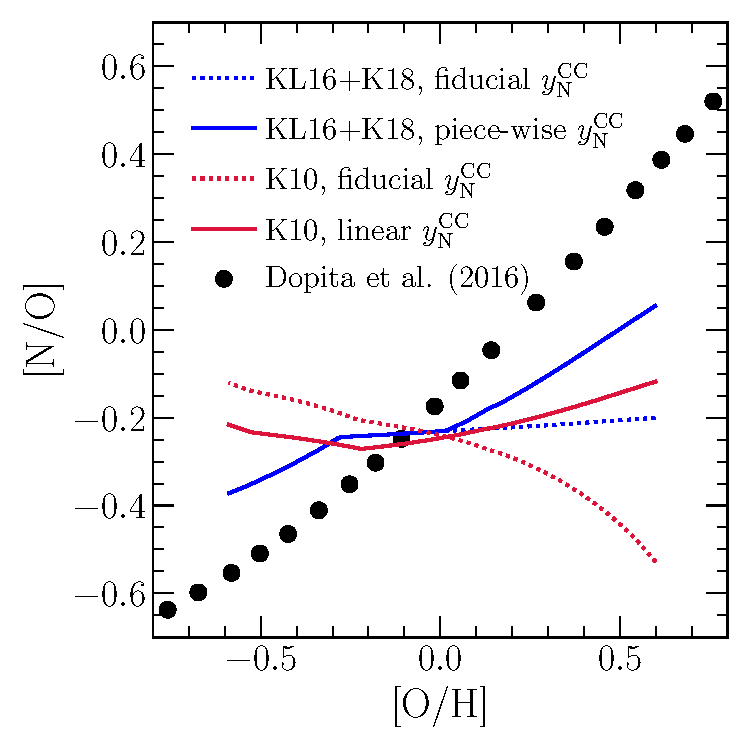
\includegraphics[scale = 0.45]{no_oh_predictions_karakas.pdf}
\caption{
\textbf{Left}: The present-day gas-phase~\ohno~relation predicted by our
model with each of the four AGB star yield tables predict by stellar evolution
models discussed in~\S~\ref{sec:yields:agb}, colour-coded according to the
legend.
We include the~\citet{Dopita2016} empirical relation as the observational
benchmark.
\textbf{Middle}: The same as the left panel, but for a case where we
artificially amplify the~\cristallo~yields by a factor of 3 and
the~\ventura~yields by a factor of 2.
We show our fiducial model using the linear AGB star yields with a slope
of~$\xi = 9\times10^{-4}$ in a solid purple line.
The black dashed line shows a model in which the~\cristallo~yields are
unmodified but SN yields and the outflow mass loading factor are lowered by a
factor of 3 (see discussion in~\S~\ref{sec:results:yields:variations}).
\textbf{Right}: The same as the left panel, but comparing the predictions made
by the~\karakasten~and~\karakas~yields with our fiducial value of
$y_\text{N}^\text{CC}$ (dotted lines, same as left-hand panel) to those with
alternate forms of~$y_\text{N}^\text{CC}$ (solid lines; see
equations~\ref{eq:broken_yncc} and~\ref{eq:linear_yncc} and discussion
in~\S~\ref{sec:results:yields}).
We show all predictions with our post-processing migration prescription (see
discussion in~\S~\ref{sec:multizone}).
}
\label{fig:no_oh_predictions}
\end{figure*}

We use the~\citet{Dopita2016}~\ohno~relation, which is inferred by fitting
local stars and HII regions spanning a wide range of~\oh, as our observational
benchmark.
As seen in Fig.~\ref{fig:no_oh_observed}, the~\citet{Pilyugin2010} ``ONS''
calibration leads to a steeper relation at high~\oh.
Following~\citet{Vincenzo2021}, we adopt the~\citet{Dopita2016} relation
because it agrees well with the trends found for APOGEE disc stars and with
results for MaNGA galaxies~\citep[][see
Fig.~\ref{fig:no_oh_observed}]{Belfiore2017}.
None the less, uncertainties in the observed trends remain, and adopting a
significantly different relation would lead to different conclusions about the
metallicity dependence of N yields.
To make the comparison between different yield models more clear, we neglect
the impact of stellar migration on enrichment rates and make use of the
post-processing migration prescription in this section (see discussion
in~\S~\ref{sec:multizone}).
In each panel of Fig.~\ref{fig:no_oh_predictions}, black points show
the~\citet{Dopita2016} trend.
The purple curve in the middle panel shows the prediction of our fiducial
(linear) yield model, which achieves excellent agreement with this
observational benchmark.
\par
In the left panel of Fig.~\ref{fig:no_oh_predictions}, we compare our model
predictions with each of the AGB star yield tables predicted from stellar
evolution models (see Fig.~\ref{fig:agb_yield_models} and discussion
in~\S~\ref{sec:yields:agb}).
% With no changes to the~\citet{Johnson2021} parametrization of the model, all
% four AGB star yield tables fail to reproduce the~\ohno~relation as observed.
% {\color{red}
Swapping our linear yields (equation~\ref{eq:linear_yield}) out from the
fiducial model for any of these AGB yields taken from the literature results
in a failure to reproduce the observed~\ohno~relation.
% }
The~\cristallo~and~\ventura~yields are able to reproduce the qualitative trend,
but with an incorrect normalization.
The~\karakasten~and~\karakas~yields, on the other hand, fail to reproduce
the steadily sloped increase of~\no~with~\oh.
The inverse dependence of~\no~with~\oh~predicted by the~\karakasten~AGB star
yields can be understood by the interaction between TDU and HBB (see discussion
in~\S~\ref{sec:yields:agb}).
Both effects are stronger at low metallicity, and since all of
the~\karakasten~stars experiencing HBB also experience TDU (see their table 1),
such a result is unsurprising.
This is also true for the~\karakas~yields, but that model predicts a
relatively flat~\ohno~relation because of updated model inputs regarding
opacity and mass loss and the impact this has on~\Nfourteen~yields (see
discussion in~\S~\ref{sec:yields:agb}).

\subsubsection{Variations in SN Yields and Outflows}
\label{sec:results:yields:variations}

In order to successfully reproduce the observations with
the~\cristallo~and~\ventura~yields, we find that we must artificially amplify
them by factors of~$\sim$3 and~$\sim$2, respectively.
We illustrate the results of these modified yield models and for our fiducial
linear model with a normalization of~$\xi = 9\times10^{-4}$ in the middle panel
of Fig.~\ref{fig:no_oh_predictions}.
Although the~\ventura~model predicts an~\ohno~relation that is slightly
shallower than the~\citet{Dopita2016} data, the predictions are
reasonably within the scatter seen in Fig.~\ref{fig:no_oh_observed}.
\par
As an alternative to amplifying the~\cristallo~and~\ventura~yields, we find
good agreement with the observed relation if we instead lower our SN yields
of N and O.
The equilibrium~\no~ratio is largely determined by the IMF-averaged N and O
yields, so lowering~\ycc{O}~has much the same effect on~\no~as raising the AGB
star N yields.
However, lowering~\ycc{O}~while holding other GCE parameters fixed reduces the
O abundance at each Galactocentric radius, so the model no longer reproduces
the normalization of the observed Galactic~\oh~gradient.
We can mostly repair this second problem by also reducing the outflow mass
loading efficiencies assumed in the model.
For a constant SFR, the equilibrium O mass fraction
is~$Z_\text{O} = \ycc{O}/(1 + \eta - r)$ where~$r \approx 0.4$ is the recycling
factor~\citep{Weinberg2017}.
The black dashed curve in the middle panel of Fig.~\ref{fig:no_oh_predictions}
illustrates a model with the unmodified~\cristallo~yields,~\ycc{O}~lowered by a
factor of 3, and~$\eta$ lowered by a factor of 3 at all radii.
This model exhibits good agreement with the~\citet{Dopita2016} trend because N
and O yields are both below those of the fiducial model by the same factor.
The model reaches solar~\oh~at the solar radius, but it predicts lower~\oh~in
the inner galaxy (i.e. a reduced x-axis span in
Fig.~\ref{fig:no_oh_predictions}) because lowering~$\eta$ by a factor of 3 does
not lower~$1 + \eta - r$ by a factor of 3.
% Under this alternate parametrization, the~\ohno~relation is also in good
% agreement with the~\citet{Dopita2016} data, but it underestimates the
% normalization of the radial metallicity gradient with lower~\oh~overall.
% Because the gradient arises in our model out of the balance between yields and
% outflows (see discussion near the end of~\S~\ref{sec:multizone}), we then lower
% our outflow mass-loading factor~$\eta$ at all radii to raise the abundances back
% to empirically plausible values.
% We demonstrate this in the middle panel of Fig.~\ref{fig:no_oh_predictions}
% with the black dashed line for the unmodified~\cristallo~yields with
% both~\ycc{O} and~$\eta$ each lowered by a factor of 3.
% With weakened outflows, this model still spans a different range in~\oh~because
% the relation between~\ycc{O}, $\eta$, and the equilibrium abundance is only
% approximately one-to-one, but the predictions also exhibit good agreement with
% the~\citet{Dopita2016} measurements.
\par
Lowering our SN yields by a factor of~$2 - 3$ is plausible if a substantial
fraction of massive stars collapse directly to black holes as opposed to
exploding as SNe at the ends of their lives.
Our IMF-averaged massive star yields (see discussion in~\S
\ref{sec:yields:ccsne}) are based on a~\citet{Kroupa2001} IMF combined with SN
nucleosynthesis models in which most~$M > 8~\msun$ stars explode as a CCSN
\cite[e.g.][]{Woosley1995, Chieffi2004, Chieffi2013, Limongi2018, Nomoto2013}.
However, many massive stars may collapse to form black holes without a SN
(\citealp*{Pejcha2015, Gerke2015};~\citealp{Sukhbold2016, Ertl2016, Adams2017,
Basinger2021, Neustadt2021}).
With the explosion landscape predicted by their W18 neutrino-driven engine, the
CCSN models of~\citet{Sukhbold2016} predict~\ycc{O}~= 0.0056
\citep{Griffith2021a}, nearly three times lower than our fiducial
value.\footnote{
	This can be calculated with~\vice~using the
	\texttt{vice.yields.ccsne.fractional} function, designed to compute values
	of~\ycc{X} for various elements under a variety of assumptions.
}
Extensive black hole formation would also lower~\ycc{Fe}, and a lower
normalization of~\yia{Fe} may be compatible with observational constraints on
SN Ia rates (see discussion in~\S~\ref{sec:yields}).
% but recent results contest the validity of this assumption.
% The criteria for massive star explosions and which stars of what masses end
% their lives in ``failed supernovae'' has been a recent topic of interest from
% both theoretical~\citep[e.g.][]{Pejcha2015, Sukhbold2016, Ertl2016} and
% observational perspectives (e.g.~\citealp*{Gerke2015};~\citealp{Adams2017,
% Basinger2021}).
% Although there is presently no combination of a SN nucleosynthesis model with
% a physically motivated black hole landscape that is able to reproduce the
% observed abundance patterns~\citep{Griffith2021a}, black hole formation still
% lowers SN yields by simply not ejecting massive star envelopes to the ISM.
% With~\vice's~\texttt{vice.yields.ccsne.fractional} function, designed to
% calculate values of~\ycc{X}~for various elements (see discussion
% in~\S~\ref{sec:yields:ccsne} here and in~\S~4 of~\citealp{Griffith2021a}), we
% indeed find a value of~$\ycc{O} = 0.0056$ using the W18 explosion model from
% \citet{Sukhbold2016} compared to our fiducial value of~$\ycc{O} = 0.015$.
% Through this mechanism relating N yields to the CCSN yields of O via~\no~ratios
% and consequently to the black hole landscape, the~\cristallo~and~\ventura~models
% favor a scenario in which a substantial fraction of massive stars produce
% failed supernovae, significantly suppressing O yields by a factor of~$2 - 3$.
% If instead most massive stars successfully explode as CCSNe, these AGB star
% yields must increase by a similar factor to offset the additional O yield under
% the more explosive black hole landscape.
\par
Another alternative is to retain high~\ycc{O}~but assume that Galactic winds
preferentially remove SN products relative to AGB products. In particular,
~\citet{Vincenzo2016a} are able to reproduce the~\ohno~relation
in chemical evolution models with the~\ventura~yields by implementing a
differential wind in which outflows remove O but not N from the star forming
gas reservoir.
We find similar results for the~\ventura~yields if we simply add a portion of
the SN products (both CCSN and SN Ia) directly to the outflow, which is
otherwise composed of swept up ambient ISM with the same abundance ratios but
reduced~$\eta$.
% Because the enrichment rates are the same as in our models with lowered
% yields, we find similar results if we simply add a portion of the SN products
% (both CCSN and SN Ia) directly to the outflow while still lowering~$\eta$ at
% all radii.
If SNe are the sources of outflow-driving winds but AGB stars do not
significantly contribute, it would be reasonable to expect some portion of
the SN ejecta to be swept up by the wind; recent theoretical
\citep{Christensen2018} and observational arguments~\citep*{Chisholm2018}
indeed suggest such a scenario.

\subsubsection{Metallicity-Dependent CCSN Yields of N}
\label{sec:results:yields:yncc}

While the issue for the~\cristallo~and~\ventura~yields is one of normalization,
our models with the~\karakasten~or~\karakas~AGB yields predict a
qualitatively incorrect trend of~\no~with~\oh.
This discrepancy cannot be repaired by changing~\ycc{O}.
However, the N yield is the sum of CCSN and AGB star contributions, so it is
reasonable to ask if plausible changes to the metallicity dependence of the
CCSN yield can compensate.
Motivated by the observed~\no~plateau at low metallicity and by the predictions
of rotating massive star models, we have thus far assumed a
metallicity-independent~$\ycc{N} = 3.6\times10^{-4}$.
However, the non-rotating CCSN models of~\citet{Nomoto2013} suggest
that~\ycc{N}~may increase at super-solar metallicity (see
Fig.~\ref{fig:agb_yield_models}).
We therefore construct the following parametrization for use with
the~\karakas~AGB star yields:
\begin{equation}
\ycc{N} = (3.6\times10^{-4})\max\left(1, \frac{Z}{Z_\odot}\right).
\label{eq:broken_yncc}
\end{equation}
Using this yield combination in our GCE model produces the blue solid curve
in the right panel of Fig.~\ref{fig:no_oh_predictions}.
While agreement with the~\citet{Dopita2016} trend is somewhat improved, this
model is still far from the empirical~\ohno~relation.
Achieving agreement while using the~\karakas~yields would require still higher
CCSN yields at~$Z > Z_\odot$ and somewhat lower CCSN yields at~$Z < Z_\odot$.
\par
Because the~\karakasten~AGB model predicts a high N yield at low metallicity
(Fig.~\ref{fig:ssp}), we combine it with the predicted yields of the
non-rotating CCSN models from~\citet{Limongi2018}, which we approximate as
\begin{equation}
\ycc{N} = (3.6\times10^{-4})\left(\frac{Z}{Z_\odot}\right)
\label{eq:linear_yncc}
\end{equation}
(diagonal dotted line in Fig.~\ref{fig:n_cc_yields}, left).
This combination produces the red solid line in the right panel of
Fig.~\ref{fig:no_oh_predictions}.
Although the discrepancy with the~\citet{Dopita2016} trend is somewhat reduced,
this model still underpredicts~\no~at~$Z > Z_\odot$ and overpredicts~\no~at
$Z < Z_\odot$ by large margins.
\par
We conclude that the metallicity dependence of N yields predicted by
the~\karakas~and, especially,~\karakasten~AGB models are empirically
untenable unless massive star yields are far from theoretical expectations.
The implications for stellar astrophysics are uncertain, but inspection of
Fig.~\ref{fig:agb_yield_models} suggests that the problem of these AGB star
models originates in the coexistence of TDU and HBB over a substantial
mass range (M~$\gtrsim 4~\msun$): in both models, every star that experiences
HBB also experiences TDU.

\subsubsection{Summary}
\label{sec:results:yields:summary}
The gas-phase~\ohno~relation in the Milky Way disc predicted by our GCE model
agrees well with the~\citet{Dopita2016} trend characterizing local stars and
HII regions if we assume a metallicity-independent~$\ycc{N} = 3.6\times10^{-4}$
as suggested by rotating massive star models~\citep{Limongi2018} and the linear
model of AGB yields in equation~\refp{eq:linear_yield}
with~$\xi = 9\times10^{-4}$.
Reproducing the empirical trend with the~\cristallo~(\ventura) AGB yields
requires renormalizing those yields by a factor of 3 (2) or, alternatively,
lowering the assumed CCSN O yield~\ycc{O}~and N yield~\ycc{N}~by the same
factor.
Lowering~\ycc{O}~could be physically justified if a large fraction of massive
stars collapse to black holes without producing CCSNe, and it may be
empirically tenable in a model where~\ycc{Fe},~\yia{Fe}, and outflow mass
loading efficiencies~$\eta$ are all lowered by a similar factor.
The metallicity dependence of AGB star yields predicted by
the~\karakasten~or~\karakas~models, flat or even declining with increasing
metallicity, is difficult to reconcile with the observed~\ohno~trend.

\subsection{Metallicity Dependence vs. Age Dependence}
\label{sec:results:t_z_dep_comp}

% fig 7 
\begin{figure}
\centering
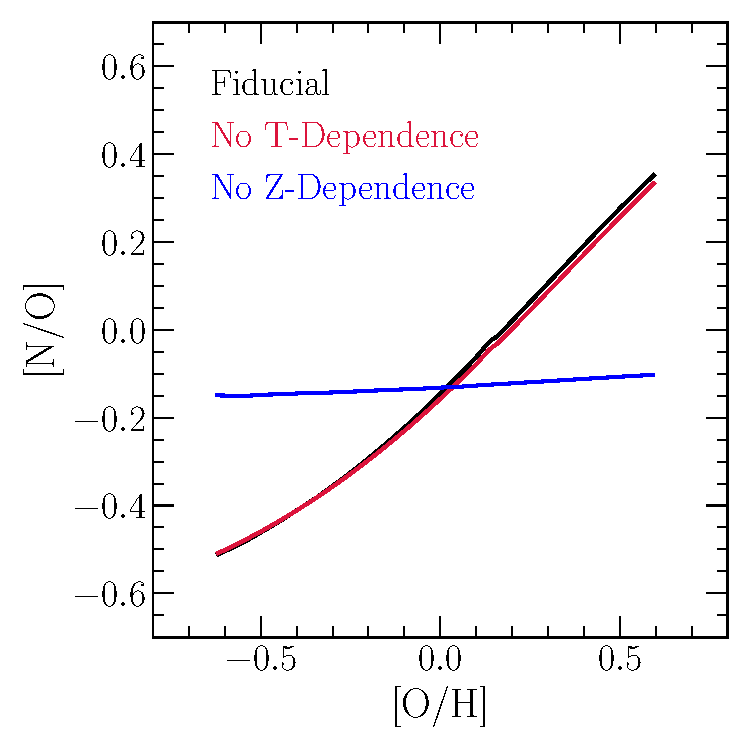
\includegraphics[scale = 0.6]{t_z_dep_comp.pdf}
\caption{
A comparison between our fiducial model with post-processing migration (black)
and variations with the time dependence (red) and metallicity dependence 
removed (blue).
To remove the time dependence, we pre-compute the AGB star yields of N from
13.2 Gyr old stellar populations as a function of metallicity as in the right
panel of Fig.~\ref{fig:ssp}, then incorporate this into the prompt CCSN yields
and set the delayed AGB star contribution to zero.
To remove the metallicity dependence, we evaluate the yields at our assumed
solar metallicity of~$Z = 0.014$ at all timesteps.
}
\label{fig:t_z_dep_comp}
\end{figure}

% Despite predicting a different mass dependence for~\yagb{N}~(see Fig.
% \ref{fig:agb_yield_models}), the renormalized~\cristallo~and~\ventura~yield
% models both reproduce the slope of the~\ohno~relation reasonably well.
Despite predicting a different mass dependence for~\yagb{N}~(see Fig.
\ref{fig:agb_yield_models}), the renormalized~\cristallo~and~\ventura~yields
both reproduce the~\ohno~relation reasonably well.
This result suggests that the metallicity dependence plays a much more
important role than the DTD in establishing this correlation.
To investigate this point further, we consider two variants of our fiducial
model: one with the dependence on stellar age (or, equivalently, stellar mass)
removed from the enrichment rate calculations, and the other with the
metallicity dependence removed.
% {\color{red}
We return to our linear AGB yield model with~$\xi = 9\times10^{-4}$, and
% }
to make this comparison more straightforward we use the post-processing
migration model (see discussion in~\S~\ref{sec:multizone}).
\par
To remove the age dependence, we simply eject the AGB star yields alongside
the CCSN yield instantaneously after a single stellar population forms.
We pre-compute the N yields from all AGB stars associated with a 13.2 Gyr old
stellar population as a function of progenitor metallicity in a similar fashion
as in the right panel of Fig.~\ref{fig:ssp}.
% {\color{red} [redacted statement about retaining the linear yield model moved
% up to first paragraph]}
%  we retain the linear yield model
% with a normalization of~$\xi = 9\times10^{-4}$ in this section.
Since~\vice~works from IMF-averaged CCSN yields assumed to be injected
instantaneously following a single stellar population's formation (see
discussion in~\S~\ref{sec:yields:ccsne}), we make use of the software's
capability to let the user specify functional forms for nucleosynthetic yields
and simply add this N yield to~\ycc{N}~and set~\yagb{N}~to zero.
In this model,~\ycc{N}~inherits a metallicity dependence from the AGB star
yields and has the exact shape of the purple curve in the right hand panel of
Fig.~\ref{fig:ssp}.
To remove the metallicity dependence, the procedure is much simpler: we simply
evaluate~\yagb{N}~at our assumed solar metallicity of~$Z_\odot = 0.014$ at all
timesteps regardless of that which is predicted for a stellar population.
In this variation, AGB star production still occurs on a DTD inherited from
the stellar mass-lifetime relation~\citep{Larson1974} and the mass dependence
of the linear yield model.
\par
We illustrate these predictions in Fig.~\ref{fig:t_z_dep_comp}.
The~\ohno~relation from the model with no age dependence is nearly identical to
the prediction found in our fiducial model, while the prediction with no
metallicity dependence is considerably different.
% This indicates that the metallicity dependence indeed plays a much larger role
% than the DTD in establishing the overall shape of the~\ohno~relation.
This result is rather unsurprising given the short characteristic timescales of
N production ($\sim$250 Myr, see the middle panel of Fig.~\ref{fig:ssp}).
Mathematically, there is little difference in the enrichment rates if all of a
stellar population's N is produced immediately as opposed to from a prompt,
sharply declining DTD.
The metallicity dependence, however, is paramount to the~\ohno~relation, which
is expected given the results in Fig.~\ref{fig:agb_yield_models} and consistent
with previous arguments that the increase in~\no~at high~\oh~is a consequence
of secondary N production~\citep{VilaCostas1993, vanZee1998, Henry1999,
PerezMontero2009, Berg2012, Pilyugin2012, Andrews2013, HaydenPawson2021}.
Fig.~\ref{fig:t_z_dep_comp} implies that the gas-phase~\ohno~relation offers
little if any constraining power over the mass dependence of N yields from
AGB stars.

\subsection{Comparison to Stellar Abundances in the Milky Way Disc}
\label{sec:results:vincenzo_comp}

% fig 8
\begin{figure}
\centering
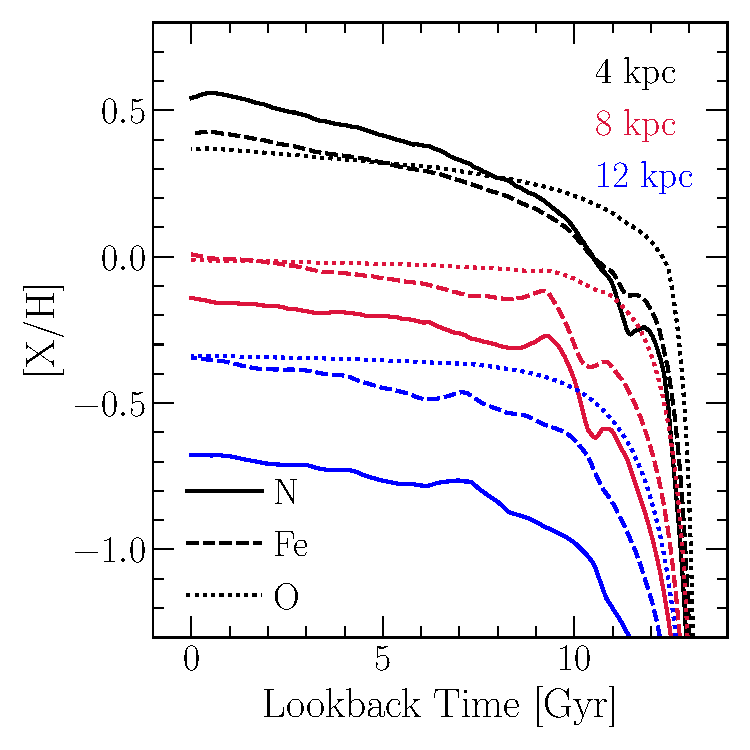
\includegraphics[scale = 0.6]{nh_feh_vs_lookback.pdf}
\caption{
\nh~(solid),~\feh~(dashed), and~\oh~(dotted) in the gas-phase as a function of
lookback time in the fiducial model at~$\rgal = 4$ (black), 8 (red), and 12 kpc
(blue).
}
\label{fig:nh_feh_vs_lookback}
\end{figure}

% fig 9
\begin{figure*}
\centering
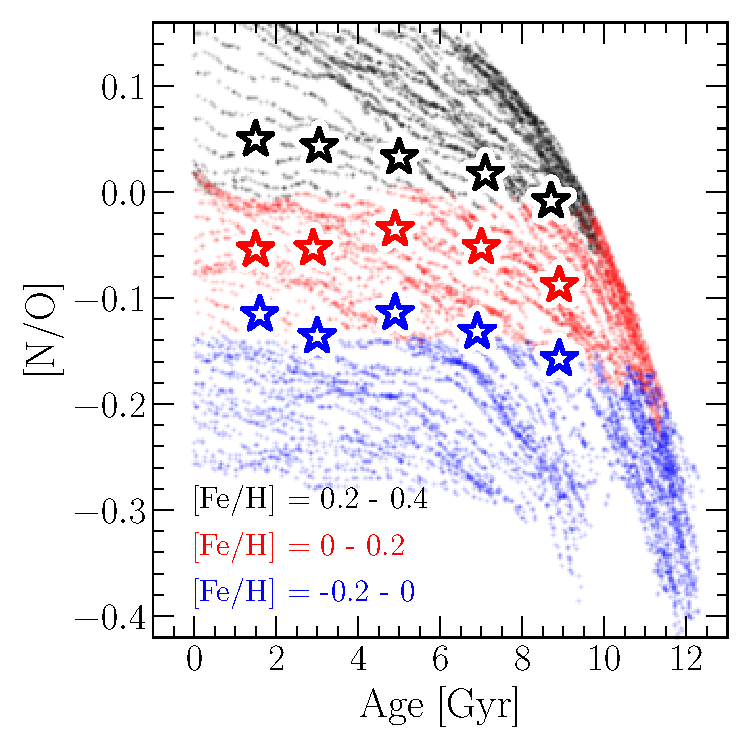
\includegraphics[scale = 0.6]{no_vs_age.pdf}
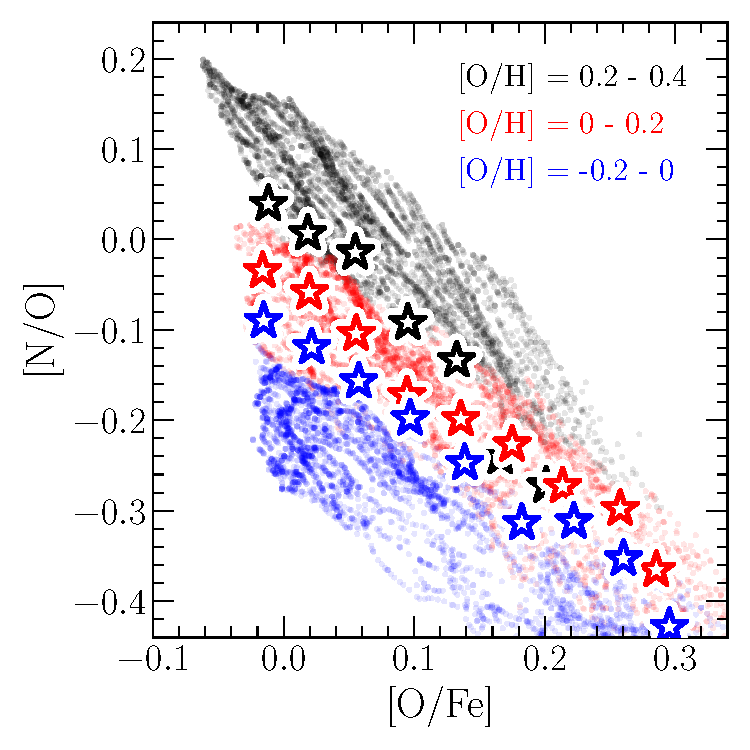
\includegraphics[scale = 0.6]{no_vs_ofe.pdf}
\caption{
\textbf{Left}:~\no~as a function of stellar age for 5000 stars randomly
sampled from our model stellar populations in three bins of~\feh~(coloured 
points).
Stars quantify the median trend in~\no~with age using N abundances corrected
for internal mixing processes reported by~\citet{Vincenzo2021} in the same
bins of~\feh.
\textbf{Right}: The same as the left panel, but instead showing~\no~as a
function of~\ofe~in bins of~\oh.
}
\label{fig:vincenzo_comp}
\end{figure*}

Although N abundances are typically measured in the gas-phase in external
galaxies, APOGEE~\citep{Majewski2017} has measured N abundances in large
stellar samples spanning many regions of the Milky Way.
By additionally making use of these data, we can investigate trends with
stellar age and~\ofe~at fixed metallicity.
Before comparing the predictions of GCE models to N abundances derived from
spectra of red giant samples such as APOGEE, it is essential to adjust the
measurements for internal processes known to alter the surface compositions of
stars because GCE models predict the birth abundances.
During the main sequence lifetime of M~$\gtrsim 1.3~\msun$ stars, the CNO cycle
processes much of the C and O nuclei in the core into~\Nfourteen.
When the star evolves off the main sequence, this N-rich material is mixed with
the outer convective layers, increasing the N abundance in the
photosphere~\citep{Gilroy1989, Korn2007, Lind2008, Souto2018, Souto2019}.
Using~\texttt{MESA} stellar evolution models~\citep{Paxton2011, Paxton2013,
Paxton2015, Paxton2018} with standard mixing prescriptions,~\citet{Vincenzo2021}
developed a recipe to approximate the birth abundances of C, N, and O and
applied it to the sample of APOGEE/Kepler red giants with asteroseismic mass
measurements from~\citet{Miglio2021}.
They found good agreement between the mean trend of~\no~with~\oh~for APOGEE
disc stars and the~\citet{Dopita2016} trend.
Since our fiducial model reproduces the~\citet{Dopita2016} trend over most of
its history (Fig.~\ref{fig:no_oh_timeevol}), it should also reproduce
the~\ohno~relation for APOGEE disc stars.
\par
Our models predict a correlation between N and Fe abundances in
the gas-phase which turns out to be important to understanding how the model
predictions compare to stellar abundances.
In Fig.~\ref{fig:nh_feh_vs_lookback}, we plot the evolution of~\nh,~\oh,
and~\feh~in the ISM at~$\rgal = 4$, 8, and 12 kpc in our fiducial model with
% {\color{red}
linear AGB yields (equation~\ref{eq:linear_yield}) and the diffusion migration
prescription (see discussion in~\S~\ref{sec:multizone}).
% }
% diffusion migration (see discussion in~\S~\ref{sec:multizone}).
\nh~is more correlated with~\feh~than~\oh~at all radii, and the relation
persists up to lookback times of~$\sim$10 Gyr.
This arises in part because N and Fe are both produced in significant
quantities by delayed enrichment sources while O is produced almost entirely on
short timescales by CCSNe (see discussion in~\S~\ref{sec:yields}).
Although the production timescale of N from single stellar populations is
short (see discussion in~\S~\ref{sec:yields:imf_agb}), metallicity dependent
yields require more abundant species such as O to be produced and reach an
equilibrium before N yields stabilize.
When many stellar populations are present, the bulk of the N production will
thus always follow the bulk production of more abundant species; this is 
qualitatively similar to what~\citet{Johnson2020} found regarding the
production timescales of Sr and Fe.
As a consequence of both its slight delay and its metallicity-dependent
yields, N reaches its equilibrium abundance on timescales similar to Fe rather
than O.
Due to the prompt and metallicity independent nature of O enrichment,~\oh~is
near equilibrium as far back as~$\sim$10 Gyr ago while~\nh~and~\feh~are not.
\par
Combining the~\citet{Vincenzo2021}~\no~ratios with the APOGEE stellar ages
taken from~\citet{Miglio2021}, we illustrate the~\no-age relation in bins
of~\feh~as predicted by our model and measured by APOGEE in the left panel of
Fig.~\ref{fig:vincenzo_comp}.
In good agreement with the observational measurements, the model predicts
the~\no-age relation to be relatively flat in bins of~\feh.
This arises as a consequence of the N-Fe correlation and the fast approach to
equilibrium in~\oh~as discussed above (see Fig.~\ref{fig:nh_feh_vs_lookback}).
A bin in~\feh~approximately corresponds to a bin in~\nh, and by extension a bin
in~\no~as well since~\oh~is nearly constant at fixed radius up to~$\sim$10 Gyr
ago.
% With uncorrected N abundances,~\citet{Vincenzo2021} demonstrate that the~\no-age
% relation exhibits a significant negative slope at fixed~\feh~(see their Fig. 7),
% indicating that we would have erroneously found a tension between our model and
% the observations if we had used uncorrected measurements.
\par
In the right panel of Fig.~\ref{fig:vincenzo_comp}, we compare our model
predictions to the~\no-\ofe~relation at fixed~\oh~reported by
\citet{Vincenzo2021}.
The model correctly predicts a significant inverse relationship
between~\no~and~\ofe.
This is again a consequence of the N-Fe correlation demonstrated in
Fig.~\ref{fig:nh_feh_vs_lookback}:~\nh~increases with~\feh, so at
fixed~\oh,~\no~increases as~\ofe~decreases.
This is another important success of our model.
\citet{Vincenzo2021} demonstrate that high [$\alpha$/Fe] and low [$\alpha$/Fe]
disc populations show a dichotomy in~\no.
The~\citet{Johnson2021} GCE model produces a broad but continuous [$\alpha$/Fe]
distribution rather than the bimodal distribution found in previous works
\citep[e.g.][]{Hayden2015, Vincenzo2021b}, but Fig.~\ref{fig:vincenzo_comp}
suggests that a model tuned to produce the [$\alpha$/Fe] bimodality would also
produce a dichotomy in~\no.
\par
Quantitatively, our model slightly underpredicts~\no~in the lower metallicity
bins in both panels of Fig.~\ref{fig:vincenzo_comp}.
In general, our model occupies a noticeably wider range in~\no~than do the
\citet{Vincenzo2021} measurements at all ages and all~\ofe.
This could be a sign that the AGB star yields of N in our fiducial model scale
slightly too strongly with the total metallicity~$Z$.
Since our fiducial model assumes an exactly linear scaling of the N yield
with~$Z$ (see equation~\ref{eq:linear_yield}), this suggests that perhaps a
slightly sub-linear scaling would be more accurate, but only barely because
the discrepancies in Fig.~\ref{fig:vincenzo_comp} are at the~$\sim$0.1 dex
level.
\par
Although we demonstrate in~\S~\ref{sec:results:t_z_dep_comp} that the
metallicity dependence of the yield plays the strongest role in establishing
the~\ohno~relation, the DTD plays a significant role in shaping the stellar
abundances.
In the model in which AGB nucleosynthetic yields are injected instantaneously
along with CCSN products, the N-Fe correlation described above is no longer
present.
Instead, N approaches equilibrium on much faster timescales, resulting in it
being much more correlated with O than Fe, and the resulting~\no-age relation
is positively sloped at fixed~\feh.
This suggests that the DTD may play a minimal role in establishing gas-phase
abundances but is important in shaping stellar abundances.
We find additional discrepancies if we instead attribute the delayed N
production to a metallicity-dependent SN Ia yield with the same~$t^{-1.1}$ DTD
that we adopt for Fe.
The agreement in Fig.~\ref{fig:vincenzo_comp} suggests that our fiducial model
has a fairly accurate separation of CCSN and AGB contributions and that the
$\sim$250 Myr characteristic delay for AGB enrichment predicted by this model
is approximately correct -- instantaneous N enrichment is too fast and
$t^{-1.1}$ enrichment is too slow to match the observations.

\subsection{The Sources of Scatter in the~\ohno~Relation}
\label{sec:results:schaefer_comp}

% fig 10
\begin{figure*}
\centering
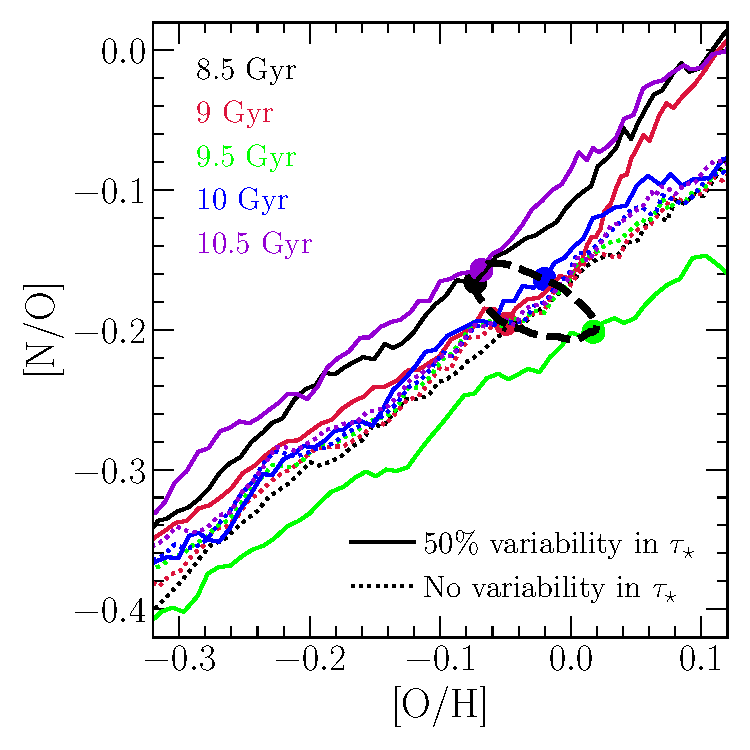
\includegraphics[scale = 0.44]{no_oh_sfevar.pdf}
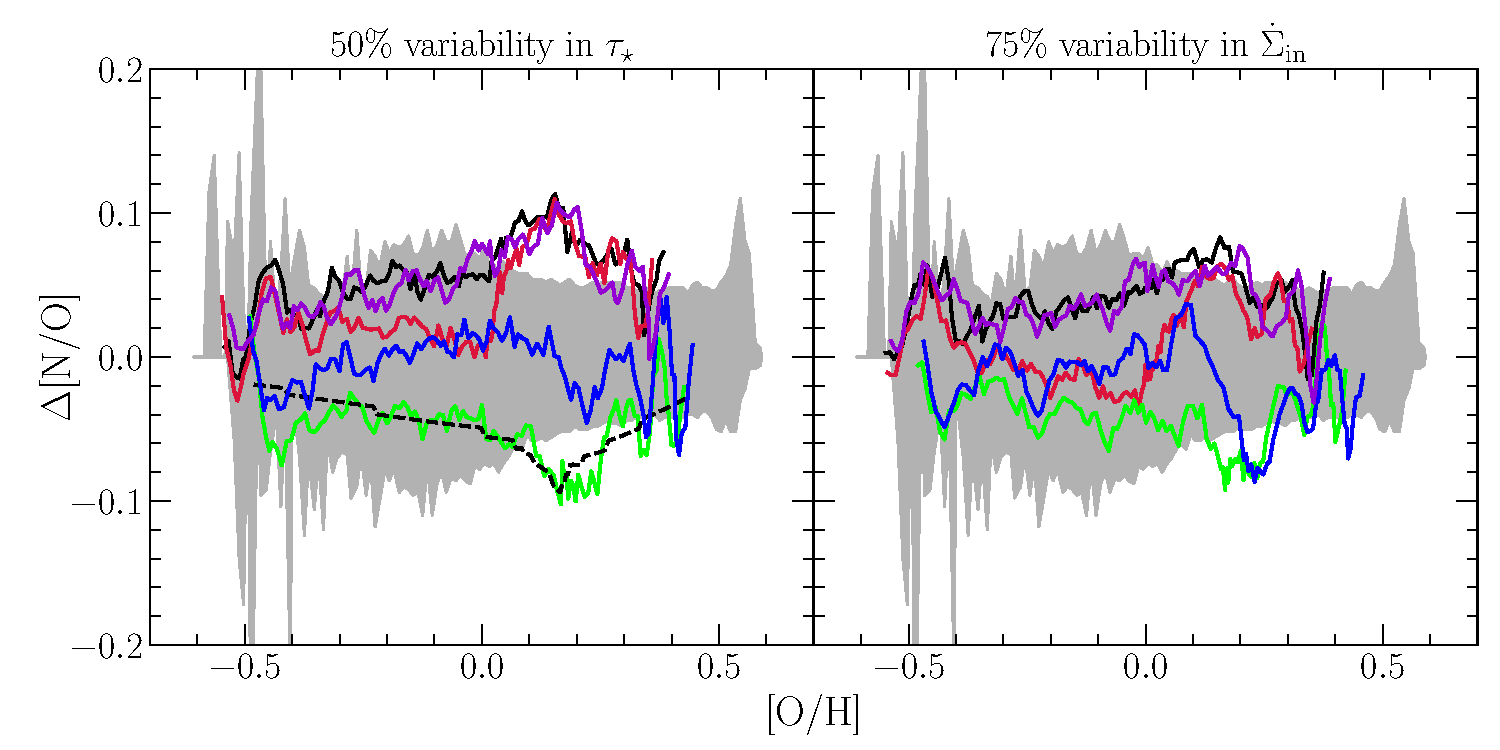
\includegraphics[scale = 0.47]{delta_no_schaefercomp.pdf}
\caption{
\textbf{Left}: One cycle of oscillations in the~\ohno~relation at
high~\oh~induced by sinusoidal variability in~$\tau_\star$ with an amplitude of
0.5 (solid coloured lines; see equation~\ref{eq:sfe_var}).
Dotted lines show the~\ohno~relation at the same five snapshots in the fiducial
model with no variability in~$\tau_\star$.
We use the diffusion migration prescription in both cases (see discussion
in~\S~\ref{sec:multizone}).
The black dashed line shows the time evolution of the abundances at~$\rgal = 8$
kpc, the approximate Galactocentric radius of the sun, with the times of each
of the five snapshots marked by a coloured point.
\textbf{Middle and Right}: For the same five snapshots in the left hand panel,
the deviation in~\no~at fixed~\oh~relative to the fiducial model for the case
with sinusoidal variability in~$\tau_\star$ at an amplitude of 0.5 (middle; see
equation~\ref{eq:sfe_var})
and with sinusoidal variability in~$\dot{\Sigma}_\star$ at an amplitude of 0.75
(right; see equation~\ref{eq:ifr_var}).
The shaded regions in both panels quantify the width of the [N/O] distribution
in~$10^{10.5} - 10^{11}~\msun$ galaxies in MaNGA taken from
\citet{Schaefer2020}.
In bins of~\oh, we place the median~\no~at~$\Delta\no = 0$, and the lower
(upper) envelope denotes the 16th (84th) percentile of the~\no~distribution.
The black dashed line in the middle panel denotes the same quantity as the
corresponding solid green line but computed from the post-processing migration
prescription, which neglects the impact of stellar migration in computing
enrichment rates (see discussion in~\S~\ref{sec:multizone}).
}
\label{fig:schaefer_comp}
\end{figure*}

\citet{Schaefer2020} demonstrate that intrinsic scatter in the
gas-phase~\ohno~relation is correlated with variations in the local SFE.
This is expected from one-zone GCE models~\citep[e.g.][]{Molla2006,
Vincenzo2016a}.
% However,~\citet{Schaefer2020} did not rule out radial migration as another
% potential source of scatter in this relation.
Although we have demonstrated in~\S~\ref{sec:results:fiducial} that the impact
of stellar migration on enrichment rates is small, it could none the less
contribute additional scatter in the observed~\ohno~relation.
Our models, taking into account the effects of migration on the
enrichment rates while allowing full control over the SFH and the SFE
through~\vice, are an ideal tool with which to address this question.
\par
To this end, we construct two variants of our fiducial model
% {\color{red}
with linear AGB yields (equation~\ref{eq:linear_yield}) and the
diffusion migration prescription (see discussion in~\S~\ref{sec:multizone}).
% }
While the fiducial model specifies the SFH~\textit{a priori} and
lets~\vice~compute the infall history~$\dot{\Sigma}_\text{in}$, here we specify
the infall history as a function of radius and time.
As we will demonstrate below, the effects of dilution play an important role in
driving variations in the~\ohno~plane in these variants, and by specifying the
infall history we have more control over the amount of dilution.
In a similar fashion as in our fiducial model, we normalize
$\dot{\Sigma}_\text{in}$ such that a stellar mass consistent with that reported
by~\citet{Licquia2015} arises from the simulation.
% {\color{red}
All other evolutionary parameters are the same as described
in~\S~\ref{sec:multizone}.
% }
% All other evolutionary parameters are the same as in the~\citet{Johnson2021}
% fiducial model (see discussion in~\S~\ref{sec:multizone} for details).
\par
In the first variant, the SFE exhibits 50\% sinusoidal oscillations with time
over 2 Gyr periods:
\begin{equation}
\tau_\star(\rgal, t) = \tau_{\star,\text{J21}}(\rgal, t)
\left(1 + 0.5\sin\left(\frac{2\pi t}{2~\text{Gyr}}\right)\right).
\label{eq:sfe_var}
\end{equation}
The infall rate is constant in each ring with a value determined by normalizing
to the present day stellar mass and stellar surface density gradient of the
Milky Way.
Our choice of a 50\% amplitude is comparable to the observationally derived
scatter in molecular gas depletion times according to multiple measurement
methods (see figs. 4 and 5 of~\citealp{Tacconi2018} and references therein).
Furthermore, variations in the SFE are of similar magnitude in~\hsim, the
galaxy from which our model's migration history is drawn.
In the second variant, the SFE is constant and the infall rate oscillates with
a 75\% amplitude about its value in the first variant:
\begin{equation}
\dot{\Sigma}_\text{in}(\rgal, t) = \langle\dot{\Sigma}_\text{in}\rangle
\left(1 + 0.75\sin\left(\frac{2\pi t}{2~\text{Gyr}}\right)\right).
\label{eq:ifr_var}
\end{equation}
The amplitude of 75\% is chosen such that the ensuing variability in the SFR is
of similar magnitude between the two models ($\sim$40\%).
We additionally run a model in which neither the accretion rate nor the SFE
oscillate, replacing the fiducial model used in previous sections with this
constant infall model.
Otherwise, the evolutionary differences beyond simple oscillations complicate
the comparison.
\par
These variant models characterize evolutionary pathways in which star formation
is more episodic than previously explored.
% In the first, this arises out of internal processes at a constant accretion
% rate from the intergalactic medium, and may be caused by, e.g., star formation
% itself inducing a tug-of-war between heating and cooling processes.
% In the second, internal processes are suppressed and the episodic nature instead
% arises out of clumpy accretion events.
In a real galaxy, variability in the SFE and the SFR is likely non-sinusoidal
and not with constant amplitude.
A sample of galaxies will have different amplitudes and be seen at different
phases in their variability, and the impact of this on their N and O abundances
will present as intrinsic scatter in a sufficiently large sample.
By comparing models with and without reasonable amounts of variability in these
quantities while taking into account radial migration, we can assess which
quantities impact abundances more strongly and are thus the more likely causes
of intrinsic scatter in the observed~\ohno~relation.
\par
In the left panel of Fig.~\ref{fig:schaefer_comp}, we plot the predicted
gas-phase~\ohno~relation for five snapshots covering one cycle of fluctuations
induced by variability in~$\tau_\star$ according to equation~\refp{eq:sfe_var}.
This model predicts a~$\sim$0.1 dex dynamic range in~\no~at fixed~\oh, whereas
the constant model with no variability in~$\tau_\star$ predicts the relation
to be quite steady over this time interval.
This suggests that stellar migration, present in both the constant model and
this oscillatory variant, does not induce significant variability in
the~\ohno~plane; however, we demonstrate below that its effects are none the
less non-negligible.
The minimal impact of stellar migration traces back to the timescales of N
production from single stellar populations (see Fig.~\ref{fig:ssp} and
discussion in~\S~\ref{sec:yields:imf_agb}): with most N production occurring
within~$\sim$250 Myr of a stellar population's formation, most stars will not
migrate far from their birth radius by the time they produce most of their N,
and the resulting impact on abundances is small.
\par
The behavior in the~\ohno~plane predicted by the oscillatory SFE variant
is driven by the tug-of-war between dilution and re-enrichment
associated with oscillations in~$\tau_\star$.
When star formation quickens, O production increases in proportion.
The ISM abundance and consequently the N yields increase as well.
Because of the slight but none the less finite delay-time of its production by
AGB stars, the N enrichment rate lags slightly behind O.
\no~therefore decreases, and the ISM moves down and to the right in
the~\ohno~plane.
When star formation eventually slows, O production again follows suit.
The N enrichment rate, as before, lags slightly behind, and~\no~increases; the
ISM therefore moves up and to the left in the~\ohno~plane.
The result is an anti-clockwise loop, which we illustrate for the solar circle
with a black dashed line in the left panel of Fig.~\ref{fig:schaefer_comp}.
The effect is generally larger in~\oh~than in~\no~($\sim$0.1 dex versus
$\sim$0.05 dex in this example) because dilution affects
both~\oh~and~\nh~similarly.
In the model with oscillations in~$\dot{\Sigma}_\text{in}$, we find that
qualitatively similar processes drive the evolution in abundances, but there
are interesting differences in detail which we discuss below in the context of
scatter in the observed trend.
\par
In the middle and right panels of Fig.~\ref{fig:schaefer_comp}, we plot the
scatter in the gas-phase~\ohno~relation inferred observationally by
\citet{Schaefer2020}.
Using data from the MaNGA IFU survey~\citep{Bundy2015}, they measure N and O
abundances in 709,541 spaxels across 6,507 unique galaxies spanning
$10^9 - 10^{11}~\msun$ in stellar mass.
Since our model is appropriate for Milky Way mass galaxies, we focus our
comparison on the~$M_\star = 10^{10.5} - 10^{11}~\msun$ mass range
\citep{Licquia2015}, which cuts our sample sample to 197,787 individual N and O
measurements from the MaNGA IFU spaxels.
In narrow bins of~\oh, we then compute the 16th, 50th, and 84th percentiles of
the~\no~distribution.
Placing the median~\no~at~$\Delta\no = 0$, the shaded regions above and below
0 in Fig.~\ref{fig:schaefer_comp} denote the difference between 16th and 84th
percentiles of the distribution in each~\oh~bin.
\par
We compare both of our oscillatory variants to the width of the~\no~distribution
by over-plotting the difference in~\no~at fixed~\oh~between our oscillatory
models and their constant counterpart (i.e. the vertical offset between the
solid and dotted lines in the left panel, and the equivalent thereof for the
oscillatory~$\dot{\Sigma}_\text{in}$ model).
Both models produce offsets in~\no~at fixed~\oh~which, as discussed above,
arise as consequences of dilution, and the offsets are generally consistent
with the width of the relation derived observationally by~\citet{Schaefer2020}.
This supports their argument that variations in the local SFE can drive
intrinsic scatter in the~\ohno~relation, but the effects of stellar migration
are still non-negligible.
We demonstrate this by comparing the green solid line in the middle panel for
the~$t = 9.5$ Gyr snapshot to the black dashed line denoting the same quantity
with post-processing migration (see discussion in~\S~\ref{sec:multizone}).
While some of the features in~$\Delta\no$ as a function of~\oh~can be
attributed to the difference in GCE parameters, stellar migration
affects~\no~ratios with an amplitude of~$\sim$0.05 dex (see also
Fig.~\ref{fig:no_oh_timeevol} and discussion in~\S~\ref{sec:results:fiducial}).
Although this is smaller than the impact of oscillations in either~$\tau_\star$
or~$\dot{\Sigma}_\text{in}$ ($\sim$0.1 dex), it is none the less significant
compared to the width of the~\citet{Schaefer2020} distributions, also at
the~$\lesssim$0.1 dex level; this suggests that stellar migration is a
subdominant but non-negligible source of scatter.
\par
In general, variability in~$\tau_\star$ impacts abundances more strongly than
variability in~$\dot{\Sigma}_\text{in}$.
Fig.~\ref{fig:schaefer_comp} shows similar changes in~\no~at fixed~\oh~in both
of our oscillatory variants, but it requires an amplitude of 75\% in accretion
rates to achieve the same~$\Delta\no$ as an amplitude of 50\% in the SFE.
This weaker impact arises out of an abundance response that is much
more~\textit{along} the~\ohno~relation rather than~\textit{against} it as in the
oscillatory~$\tau_\star$ model (see the black dashed line in the left panel of
Fig.~\ref{fig:schaefer_comp}).
Both~\oh~and~\nh~vary with larger amplitudes in the variable infall model due to
episodes of enhanced and suppressed accretion, but the effects of dilution
on~\nh~are amplified by the combination with metallicity-dependent yields.
As a result,~\nh~varies with a larger amplitude than~\oh, whereas the opposite
is the case in the oscillatory~$\tau_\star$ model.
Consequently,~\no~increases rather than decreases with increasing~\oh, and
changes in~\no~at fixed~\oh~are smaller.
In the context of the observational results~\citep{Schaefer2020}, this suggests
that different~\no~ratios at fixed~\oh~are less likely to reflect changes in
the accretion rate and more likely to reflect variations in the internal
properties of the star forming ISM, such as the thermal state or the pressure,
quantities which here get folded into~$\tau_\star$.

\subsection{The~\ohno~Relation as an Equilibrium Phenomenon}
\label{sec:results:ohno_equilibrium}

As shown by~\citet{Weinberg2017}, under generic conditions the abundances of a
one-zone GCE model with continuing gas infall evolve to an equilibrium, in
which new metal production is balanced by dilution and by the loss of ISM
metals to star formation and outflows.
Fig.~\ref{fig:no_oh_timeevol} shows that the~\no~ratio at a given radius in our
multi-zone GCE model approaches an equilibrium after~$t \approx 5$ Gyr.
Fig.~\ref{fig:t_z_dep_comp} further shows that the~\ohno~relation that emerges
in our model is driven by the metallicity dependence of the N yield, with the
time-delay of AGB enrichment having minimal impact.
This indicates that -- for the purposes of computing the equilibrium abundance
of N -- the AGB star DTD can be neglected, assuming instantaneous production as
in~\S~\ref{sec:results:t_z_dep_comp}.
This allows analytic solutions to the~\no~ratio that will arise at a
given equilibrium~\oh.
% It is therefore useful to apply insights from analytic models to the origin of
% this relation, extending our discussion
% from~\S~\ref{sec:results:yields:variations}.
\par
For an exponential SFH,~$\dot{M}_\star \propto e^{-t/\tau_\text{SFH}}$, with
instantaneous enrichment and recycling of an element X with IMF-averaged
yield~$y_\text{X}$, the equilibrium ISM mass fraction is
\begin{equation}
Z_\text{eq,X} = \frac{y_\text{X}}{1 + \eta - r - \tau_\star/\tau_\text{SFH}},
\label{eq:zeq}
\end{equation} 
where (as before)~$\eta = \dot{M}_\text{out} / \dot{M}_\star$, $r \approx 0.4$
is the recycling fraction, and~$\tau_\star = M_\text{gas} / \dot{M}_\star$ is
the SFE timescale (see section~\ref{sec:multizone}).
When an element's characteristic enrichment delay time is~$\ll \tau_\text{SFH}$,
the correction to equation~\refp{eq:zeq} is very small~\citep{Weinberg2017},
which alongside Fig.~\ref{fig:t_z_dep_comp} suggests that the AGB DTD of N
enrichment can safely be neglected for these purposes.
The~\no~abundance ratio in equilibrium is then given by the ratio of the yields
with the metallicity-dependent N yield evaluated at the equilibrium O abundance:
% Therefore, it is sufficiently accurate to compute the N equilibrium abundance
% by neglecting the AGB DTD, assuming instantaneous production as
% in~\S~\ref{sec:results:t_z_dep_comp}, and taking the value given by equation
% \refp{eq:zeq} with a metallicity-dependent~\ycc{N}.
% The~\no~abundance ratio in equilibrium is then given by the ratio of the yields
% where the N yield is evaluated at the equilibrium O abundance:
% Therefore, even with a declining SFR and AGB time delay, the~\no~abundance
% ratio in equilibrium should equal the yield ratio.
% While a full time-dependent analytic solution is only possible for a
% metallicity-independent yield, to compute the equilibrium ratio we can just
% take the N yield at the metallicity implied by the O abundance.
% This argument leads to the expectation
\begin{equation}
\no_\text{eq} = \log_{10}\left(\frac{
	Z_\text{N,eq} / Z_\text{O,eq}
}{
	Z_{\text{N},\odot} / {Z_{\text{O},\odot}}
}\right) = \log_{10}\left(\frac{
	y_\text{N}(Z_\text{O,eq}) / \ycc{O}
}{
	Z_{\text{N},\odot} / Z_{\text{O},\odot}
}\right),
\label{eq:noeq}
\end{equation}
where~$y_\text{N}(Z_\text{O})$ denotes the~\textit{total} IMF-averaged N yield
(CCSN + AGB) at a given~$Z_\text{O}$ as in Fig.~\ref{fig:ssp}.
We have spot-checked this formula for each of our AGB yield models taken from
the literature against the left panel of Fig.~\ref{fig:no_oh_predictions} and
found agreement to 0.02 dex or better, slightly smaller than the impact of
stellar migration on gas-phase N abundances (see discussion
in~\S\S~\ref{sec:results:fiducial} and~\ref{sec:results:schaefer_comp}).
\par
Equation~\refp{eq:noeq} can be used to predict the~\ohno~relation for a given
set of yields.
Our fiducial AGB star yield (equation~\ref{eq:linear_yield} with
$\xi = 9\times10^{-4}$) gives an IMF-averaged yield of~$9.3\times10^{-4}$ 
at~$Z = Z_\odot$ (Fig.~\ref{fig:ssp}; see also discussion
in~\S~\ref{sec:yields}).
Applying this value (along with~$\ycc{O} = 0.015$,
$Z_{\text{N},\odot} = 6.91\times10^{-4}$, and
$Z_{\text{O},\odot} = 5.72\times10^{-3}$) to equation~\refp{eq:noeq} and
separating the massive star contribution of~$\ycc{N} = 3.6\times10^{-4}$ for
generality gives
\begin{equation}
10^{\no_\text{eq}} = 10^{\no\subcc} + (0.513)10^{\oh_\text{eq}},
\end{equation}
where~$\no\subcc = -0.7$ is our empirical CCSN ``plateau'' taken from
Fig.~\ref{fig:no_oh_observed}, for which alternate values can be computed from
choices regarding~\ycc{N} and~\ycc{O} (see discussion
in~\S~\ref{sec:yields:ccsne}).
One can also reverse engineer equation~\refp{eq:noeq} to derive the IMF-averaged
N yield required to match an empirical~\ohno~relation given a value of~\ycc{O}.
% One can also use equation~\refp{eq:noeq} to reverse engineer the IMF-averaged
% N yield required to match an empirical~\ohno~relation for a specified
% $y_\text{O}$.
% Our fiducial AGB yield (equation~\ref{eq:linear_yield} with
% $\xi = 9\times10^{-4}$) gives an IMF-averaged yield of
% $\yagb{N} = 9.4\times10^{-4}$ (Fig.~\ref{fig:ssp}) at~$Z = Z_\odot$, with a
% linear dependence on~$Z$.
% Applying this yield (and~$\ycc{N} = 3.6\times10^{-4}$,~$\ycc{O} = 0.015$,
% $Z_{\text{N},\odot} = 6.91\times10^{-4}$,
% $Z_{\text{O},\odot} = 5.72\times10^{-3}$) to equation~\refp{eq:noeq} gives
% \begin{equation}
% 10^{\no} = 0.199 + 0.519 \times 10^{\oh}
% \end{equation}
\par
This analysis sharpens the conventional understanding of why~\no~is a useful
metallicity indicator in external galaxies when~\oh~cannot be measured directly.
The relation between~\no~and~\oh~is driven by stellar astrophysics (i.e. yields)
in a way that is relatively insensitive to the SFH, SFE, or other
galactic-scale physics.
Viewing the relation from this perspective also highlights where one should be
cautious about using~\no~as a metallicity indicator.
First is in environments where the stellar yields could be substantially
different, perhaps because of differences in the IMF or in stellar rotation.
Second is in galaxies that may be far from equilibrium, e.g. because of recent
bursts of star formation or mergers diluting the ISM.
The sinusoidal star formation variations considered
in~\S~\ref{sec:results:schaefer_comp} perturb equilibrium enough to create
$\sim$0.1 dex excursions in~\no~at fixed~\oh~(Fig.~\ref{fig:schaefer_comp}).
Third is in galaxies that are too young to have reached equilibrium.
Although the~\ohno~relation of our fiducial model is within~$\sim$0.1 dex of
its final value by~$t = 5$ Gyr, it is lower at earlier times
(Fig.~\ref{fig:no_oh_timeevol}).
One-zone models with a metallicity-dependent N yield can be used to estimate
whether high-redshift galaxies are likely to have reached equilibrium based
on their SFRs, gas fractions, metallicities, and stellar masses.
Dwarf galaxies often have low SFE and might therefore reach equilibrium more
slowly.
However, these galaxies are also typically in the low-metallicity regime
where~\no~is determined by the metallicity-independent primary yields anyway.

\end{document}

